%!TEX root = ../my_thesis.tex

\appendix
\chapter{Compléments au Chapitre Premier}
\section{Détails des calculs de l'algorithme APP}\label{append:app}
Cette partie vise à démontrer l'ensemble des calculs présentés dans la section \ref{sec:BCJR}.
\subsection{Décomposition de la probabilité jointe} 
Cette décomposition est basée sur le partitionnement de la séquence reçue $\mathbf{y}$ en trois sous-séquences. La première représentant le passé $ \mathbf{y_{<k}}$, la seconde le présent $\mathbf{y_{k}} $ et enfin le futur $ \mathbf{y_{>k}}$.

Le calcul suivant est basé sur la relation de Bayes : $P(A|B) = \frac{P(A,B)}{P(B)}$ et sa version ternaire $P(A|B,C) = \frac{P(A,B|C)}{P(B|C)}$.

Aussi, sont nécessaires au déroulement de ce calcul les propriétés de Markov du treillis de l'encodeur RSC considéré. En effet :
\begin{align*}
	\hspace*{-4ex}
	P(s_{k-1}=s, s_{k}=s',\mathbf{y}) & = P(s_{k-1}=s, s_{k}=s',\mathbf{y_{<k}},\mathbf{y_{k}},\mathbf{y_{>k}})                                                                                                                             \\
	                                  & = P(\mathbf{y_{>k}}|s_{k-1}=s, s_{k}=s',\mathbf{y_{<k}},\mathbf{y_{k}})\times P(s_{k-1}=s, s_{k}=s',\mathbf{y_{<k}},\mathbf{y_{k}})                                                                 \\
	                                  & =P(\mathbf{y_{>k}}|s_{k}=s')\times P(s_{k-1}=s, s_{k}=s',\mathbf{y_{<k}},\mathbf{y_{k}})                                                                                                            \\
	                                  & =P(\mathbf{y_{>k}}|s_{k}=s')\times P(s_{k}=s',\mathbf{y_{k}}|s_{k-1}=s,\mathbf{y_{<k}})\times P(s_{k-1}=s,\mathbf{y_{<k}})                                                                          \\
	                                  & = \underbrace{P(\mathbf{y_{>k}}|s_{k}=s')}_{\beta_k(s')}\times \underbrace{P(s_{k}=s',\mathbf{y_{k}}|s_{k-1}=s)}_{\gamma_k(s,s')}\times \underbrace{P(s_{k-1}=s,\mathbf{y_{<k}})}_{\alpha_{k-1}(s)} \\
	                                  & = \alpha_{k-1}(s) \times \gamma_k(s,s') \times \beta_k(s')                                                                                                                                          
\end{align*}

\subsection{Calcul récursif de $\alpha$}
Par définition, $\alpha_{k-1}(s) = P(s_{k-1}=s,\mathbf{y_{<k}})$. Or, sachant que $\sum\limits_B P(A,B) = P(A)$ et en appliquant le théorème de Bayes,
\begin{align*}
	\hspace*{-4ex}
	\alpha_k(s) & = \sum\limits_{s'}P(s_{k}=s,s_{k-1}=s',\mathbf{y_{<k}},\mathbf{y_k})                                        \\
	            & = \sum\limits_{s'}P(s_{k}=s,\mathbf{y_k} | s_{k-1}=s',\mathbf{y_{<k}}) \times P(s_{k-1}=s',\mathbf{y_{<k}}) \\
	            & = \sum\limits_{s'}P(s_{k}=s,\mathbf{y_k} | s_{k-1}=s') \times P(s_{k-1}=s',\mathbf{y_{<k}})                 \\
	            & = \sum\limits_{s'}\gamma_k(s',s)\times \alpha_{k-1}(s')                                                     
\end{align*}
Ainsi, les valeurs de $\alpha_k(s)$ peuvent être calculées récursivement en parcourant le treillis dans l'ordre chronologique, à partir des valeurs initiales $\alpha_0(s)$ et des probabilités de transition.

\subsection{Calcul récursif de $\beta$}
En utilisant les mêmes propriétés calculatoires que pour le calcul de $\alpha$ : 
\begin{align*}
	\hspace*{-4ex}
	\beta_{k-1}(s) & = P(\mathbf{y_{>k-1}}|s)                                                             \\
	               & = \sum\limits_{s'}P(s',\mathbf{y_{k}},\mathbf{y_{>k}|s})                             \\
	               & = \sum\limits_{s'}P(\mathbf{y_{>k}} | s',s, \mathbf{y_{k}}) P(s', \mathbf{y_{k}}| s) \\
	               & = \sum\limits_{s'}P(\mathbf{y_{>k}} | s') P(s', \mathbf{y_{k}}| s)                   \\
	               & = \sum\limits_{s'}\gamma_k(s,s')\times \beta_{k}(s')                                 
\end{align*}


\subsection{Calcul de la probabilité \textit{a posteriori}}
La probabilité \textit{a posteriori} a pour expression : 
\begin{align*}
	\|\mathbf{y}_k-\mathbf{c}_k\|^2 & = (y_k^s - c_k^s)^2 + (y_k^p - c_k^p)^2                                               \\
	                                & = (y_k^s)^2 - 2  y_k^s   c_k^s +  (c_k^s)^2 + (y_k^p)^2 - 2  y_k^p c_k^p +  (c_k^p)^2 \\
	                                & = (y_k^s)^2 +   (y_k^p)^2 + 2  - 2*( y_k^s   c_k^s +  y_k^p c_k^p)                    
\end{align*}

Ainsi, \[\gamma_k(s,s') = \frac{P(m_k)}{2\pi\sigma^2}\exp\left(-\frac{ (y_k^s)^2 +   (y_k^p)^2 + 2}{2\sigma^2}\right) \exp\left(\frac{( y_k^s   c_k^s +  y_k^p c_k^p)}{\sigma^2}\right)\]

Or, la première exponentielle n'est pas dépendante de $m_k$ (ou du chemin $ s \mapsto s'$) et peut donc être supprimé du numérateur et du dénominateur dans l’expression de la probabilité \textit{a posteriori}.


\section{Détails des calculs pour les algorithmes sub-APP}\label{append:subAPP}
\subsection{Calcul des métriques}
Dans le cadre des algorithmes sub-APP, les probabilités manipulées sont transformées en métriques en prenant le logarithme népérien de celles-ci. Ainsi, nous avons :
\begin{align*}
	\tilde{\alpha}_k(s) & = \ln \sum\limits_{s'}\alpha_{k-1}(s')\times\gamma_k(s',s)                                                     \\
	                    & = \ln \sum\limits_{s'} \exp\left(\tilde{\alpha}_{k-1}(s')\right)\times\exp\left(\tilde{\gamma}_k(s', s)\right) \\
	                    & = \ln \sum\limits_{s'} \exp\left(\tilde{\alpha}_{k-1}(s') + \tilde{\gamma}_k(s', s)\right)                     
\end{align*}
Des calculs très similaires permettent d'obtenir $\tilde{\beta}_k(s)$ et $\tilde{\gamma}_k(s,s')$.

\subsection{Opérateur $\maxstar$}\label{append:maxstar}
En partant de la définition de l’opérateur $\maxstar$ et en utilisant une disjonction de cas, on obtient : 
\begin{align*}
	\maxstar(x,y) & = \ln\left(\e^x+\e^y\right)              \\
	              & =\begin{cases}                           
	\ln	\left(\e^x\left(1+\e^{y-x}\right)\right) \text{si} x>y  \\
	\ln	\left(\e^y\left(1+\e^{x-y}\right)\right) \text{si} x<y
	\end{cases}\\
	              & =\begin{cases}                           
	x + \ln\left(1+\e^{y-x}\right) \quad\text{si}\quad x>y  \\
	y+\ln\left(1+\e^{x-y}\right) \quad\text{si}\quad x<y
	\end{cases}\\
	              & =\max(x,y) +\ln\left(1+\e^{|x-y|}\right) 
\end{align*}


% Ainsi, en reprenant les définitions récursives et en substituant les probabilités par les métriques, leurs expressions deviennent : 
% \begin{align*}
% 	M^\alpha_k(s) & = \ln \sum\limits_{s'}\alpha_{k-1}(s')\times\gamma_k(s',s)                                         \\
% 	              & = \ln \sum\limits_{s'} \exp\left(M^\alpha_{k-1}(s')\right)\times\exp\left(M^\gamma_k(s', s)\right) \\
% 	              & = \ln \sum\limits_{s'} \exp\left(M^\alpha_{k-1}(s') + M^\gamma_k(s', s)\right)                     
% \end{align*}
% et 
% \[M^\beta_k(s) = \ln \sum\limits_{s'} \exp\left(M^\beta_{k+1}(s') + M^\gamma_{k+1}(s, s')\right)\]
% avec pour conditions initiales, 

% De même les LLR \textit{a posteriori} deviennent :
% \begin{align*} 
% 	L(m_k) & = \ln \sum\limits_{s,s'\in S_1} \exp\left( M^\alpha_{k-1}(s) + M^\gamma_{k}(s, s') + M^\beta_k(s') \right)       \\ 
% 	       & \quad - \ln \sum\limits_{s,s'\in S_0} \exp\left( M^\alpha_{k-1}(s) + M^\gamma_{k}(s, s') + M^\beta_k(s') \right) 
% \end{align*}
% Toutefois, ces réécritures dans le domaines logarithmiques ne permettent pas encore de réduire la complexité calculatoire. Pour ce faire, introduisons l'opérateur \[\maxstar(x,y) = \ln(\mathrm{e}^x + \mathrm{e}^y).\]
% Ainsi, les métriques précédentes deviennent : 



% Il est démontré facilement (en utilisant un disjonction de cas) que :
% \[\maxstar(x,y) = \max(x,y) + \ln(1+e^{|x-y|})\]
% \paragraph{Stabilité numérique}


\chapter{Compléments au Chapitre Deuxième}
\section{Standard CCSDS}\label{sec:annCCSDS}
Cette section présente les observations statistiques obtenues avec le standard CCSDS. La Figure \ref{fig:m_ccsds} présente 
les valeurs moyennes d'oscillations, ce pour différentes valeurs de SNR. Les Figures \ref{fig:it1_ccsds} et \ref{fig:it2_ccsds}
présentent l'évolution des oscillations au cours des itérations pour, respectivement, un taux d'erreur trame correspondant 
au seuil de convergence et un correspondant au plancher d'erreur. Finalement, les Figures \ref{fig:d1_ccsds} et \ref{fig:d2_ccsds} 
présentent la distribution normalisée des oscillations pour ces deux valeurs de SNR considérées.
\begin{figure}[tb]
	\begin{center}
	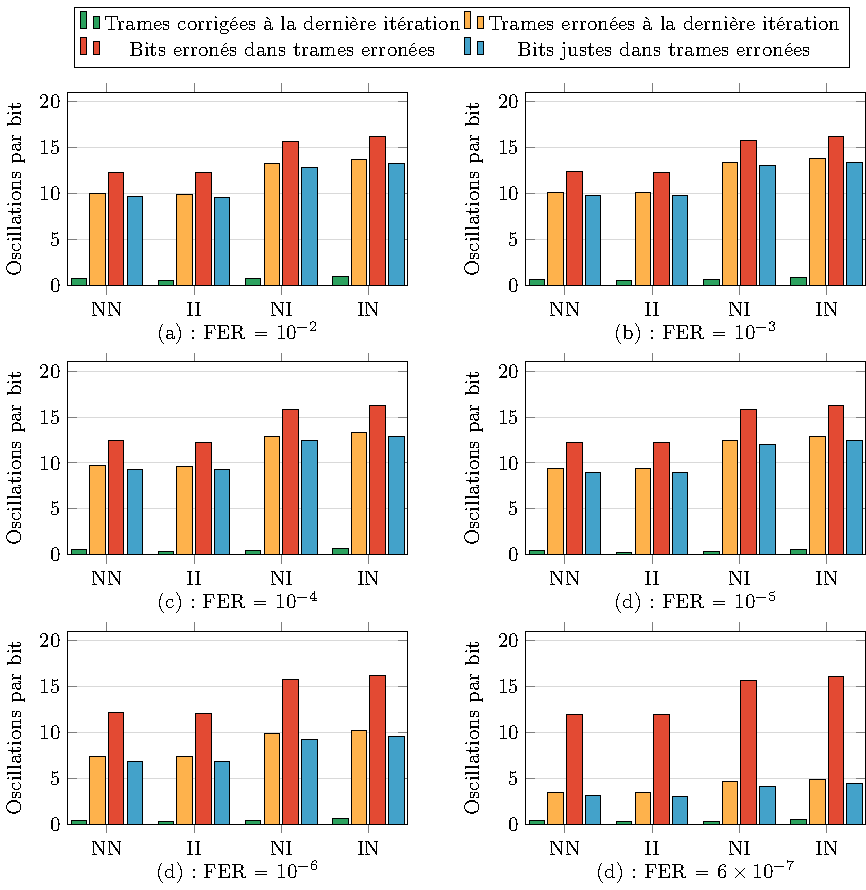
\includegraphics[width=.9\textwidth]{main/ch2_fig/tikz/m_ccsds.pdf}
	\caption{Nombre moyen d'oscillations pour différents taux d'erreurs trame cibles, turbo code du standard CCSDS (K=1784, R=1/3) \label{fig:m_ccsds}}
	\end{center}
\end{figure}

\begin{figure}[!ht]
	%\hspace*{-.7cm}	
	\begin{center}
	\includegraphics[width=.9\textwidth]{main/ch2_fig/tikz/it_ccsds10-2.pdf}
	\caption{Oscillations au cours des itérations dans le cadre du standard CCSDS (K=1784, R=1/3) pour un taux d'erreur trame de $10^{-2}$\label{fig:it1_ccsds}}
	\end{center}
\end{figure}

\begin{figure}[!ht]
	%\hspace*{-.7cm}
	\begin{center}
	\includegraphics[width=.9\textwidth]{main/ch2_fig/tikz/it_ccsds610-7.pdf}
	\caption{Oscillations au cours des itérations dans le cadre du standard CCSDS (K=1784, R=1/3) pour un taux d'erreur trame de $6\times10^{-7}$\label{fig:it2_ccsds}}
	\end{center}
\end{figure}

\begin{figure}[!ht]
	\centering
	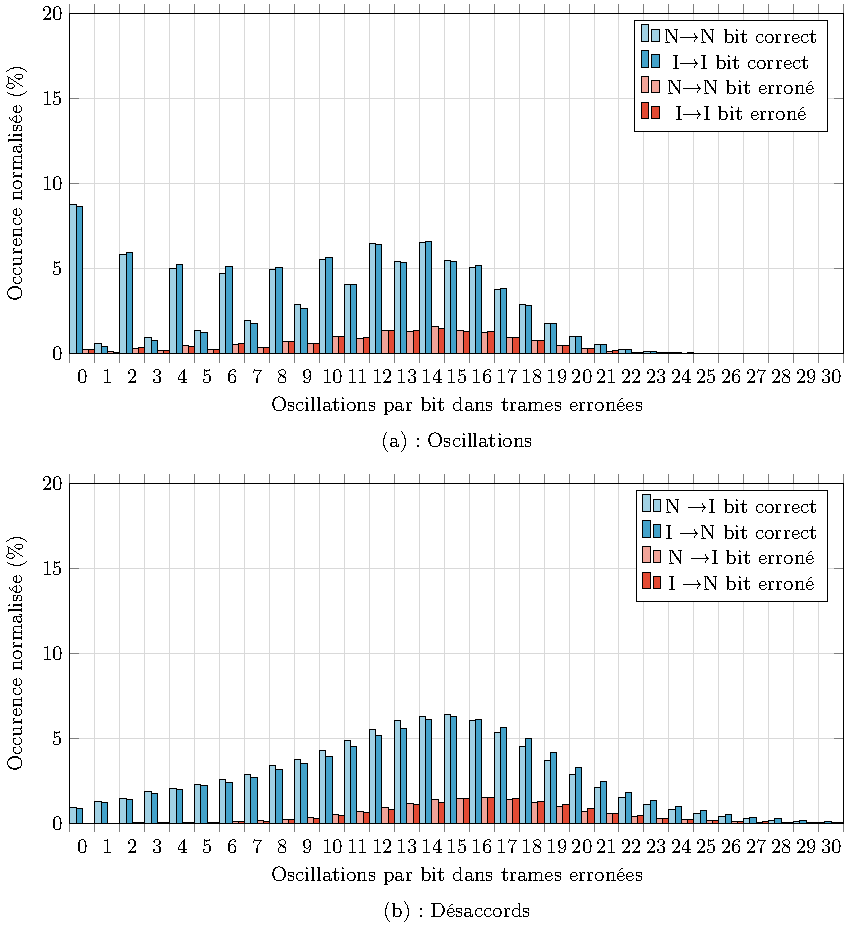
\includegraphics[width=.9\textwidth]{main/ch2_fig/tikz/d_ccsds_10-2.pdf}
	\caption{Distribution du nombre d'oscillations par bit pour un taux d'erreur trame de $10^{-2}$, pour le turbo code du standard CCSDS (K=1784, R=1/3)\label{fig:d1_ccsds}}
\end{figure}

\begin{figure}[!ht]
	\centering
	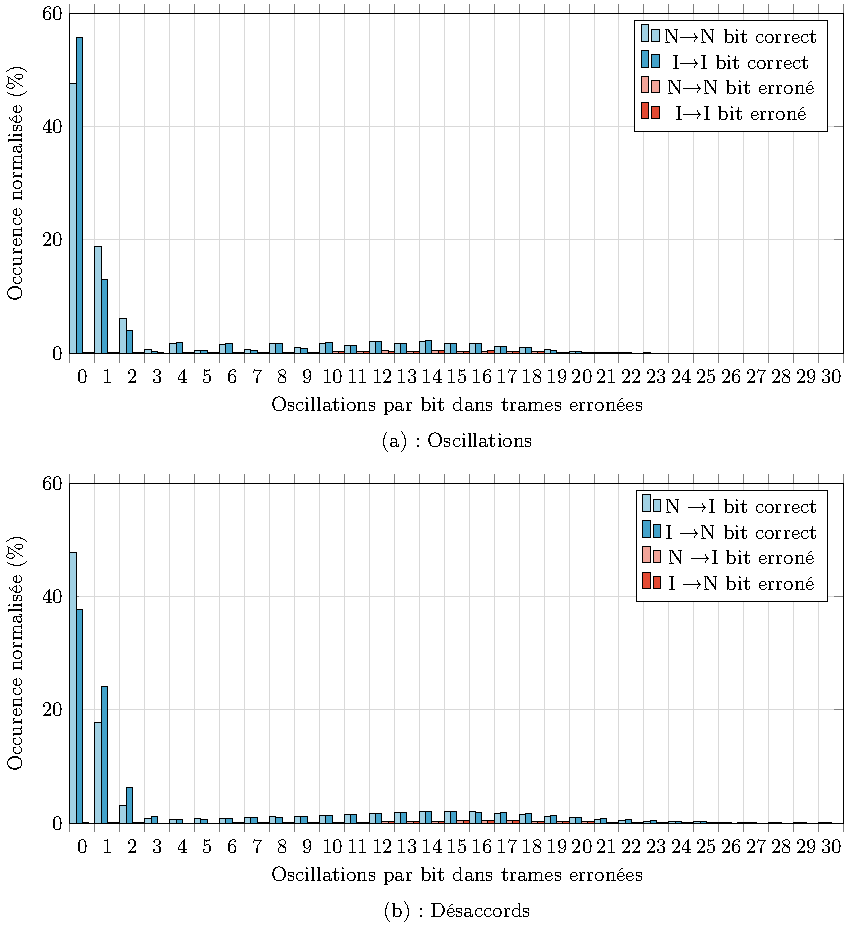
\includegraphics[width=.9\textwidth]{main/ch2_fig/tikz/d_ccsds_610-7.pdf}
	\caption{Distribution du nombre d'oscillations par bit pour un taux d'erreur trame de $6\times10^{-7}$, pour le turbo code du standard CCSDS (K=1784, R=1/3)\label{fig:d2_ccsds}}
\end{figure}


\chapter{Compléments au Chapitre Troisième}\label{sec:ann3}
\newpage
\begin{adjustbox}{angle=90}
\centering
\resizebox{1.5\textwidth}{!}{
\begin{tabular}{@{}llrrrrrrrrrrrrrrrrrrrrrrrrrrrr@{}}
\toprule
\multirow{15}{*}{\textbf{LTE}} & \multirow{3}{*}{\textbf{K=528}}  & \textbf{d} & 23 & 24 & 25 & 26 & 27 & 28 & 29 & 30 & 31 & 32 & 33 & 34 & 35 & 36 & 37   & 38   & 39    & 40   & 41  & 42  & 43   & 44   & 45   & 46  & 47   & 48  & 49  \\  
                    &    & \textbf{a} & 1  & 1  & 1  & 0  & 3  & 3  & 6  & 0  & 6  & 4  & 11 & 10 & 14 & 12 & 96   & 886  & 1421  & 45   & 123 & 156 & 192  & 227  & 140  & 55  & 285  & 52  & 62  \\
                    &    & \textbf{w} & 1  & 2  & 3  & 0  & 9  & 6  & 16 & 0  & 20 & 16 & 39 & 32 & 58 & 50 & 318  & 5268 & 12535 & 210  & 779 & 864 & 984  & 982  & 850  & 286 & 1415 & 260 & 292 \\ \cdashlinelr{2-30}
& \multirow{3}{*}{\textbf{K=1024}} & \textbf{d} & 27 & 28 & 29 & 30 & 31 & 32 & 33 & 34 & 35 & 36 & 37 & 38 & 39 & 40 & 41   & 42   & 43    & 44   & 45  & 46  & 47   & 48   & 49   &     &      &     &     \\
  &                      & \textbf{a} & 1  & 2  & 3  & 1  & 2  & 1  & 2  & 2  & 7  & 3  & 7  & 9  & 11 & 11 & 20   & 30   & 147   & 437  & 49  & 64  & 583  & 179  & 511  &     &      &     &     \\
   &                     & \textbf{w} & 1  & 4  & 9  & 2  & 6  & 2  & 6  & 6  & 21 & 12 & 27 & 32 & 43 & 44 & 78   & 142  & 719   & 1770 & 241 & 326 & 2949 & 1148 & 3407 &     &      &     &     \\ \cdashlinelr{2-30}
& \multirow{3}{*}{\textbf{K=1504}} & \textbf{d} & 25 & 26 & 27 & 28 & 29 & 30 & 31 & 32 & 33 & 34 & 35 & 36 & 37 & 38 & 39   & 40   & 41    & 42   & 43  & 44  & 45   & 46   & 47   & 48  & 49   &     &     \\
  &                      & \textbf{a} & 1  & 0  & 0  & 1  & 1  & 1  & 2  & 1  & 2  & 5  & 1  & 6  & 7  & 3  & 14   & 13   & 17    & 22   & 32  & 28  & 47   & 49   & 185  & 91  & 1414 &     &     \\
   &                     & \textbf{w} & 3  & 0  & 0  & 2  & 3  & 2  & 6  & 4  & 6  & 18 & 3  & 22 & 23 & 12 & 54   & 54   & 75    & 90   & 154 & 126 & 223  & 246  & 909  & 486 & 9696 &     &     \\ \cdashlinelr{2-30}
& \multirow{3}{*}{\textbf{K=2048}} & \textbf{d} & 27 & 28 & 29 & 30 & 31 & 32 & 33 & 34 & 35 & 36 & 37 & 38 & 39 & 40 & 41   & 42   & 43    & 44   & 45  & 46  & 47   & 48   & 49   &     &      &     &     \\
  &                      & \textbf{a} & 1  & 2  & 1  & 0  & 3  & 0  & 2  & 1  & 2  & 1  & 1  & 3  & 8  & 5  & 12   & 15   & 16    & 425  & 23  & 37  & 240  & 45   & 290  &     &      &     &     \\
   &                     & \textbf{w} & 1  & 4  & 3  & 0  & 9  & 0  & 6  & 4  & 6  & 4  & 3  & 8  & 26 & 20 & 44   & 62   & 72    & 1702 & 117 & 178 & 1180 & 230  & 1872 &     &      &     &     \\ \cdashlinelr{2-30}
& \multirow{3}{*}{\textbf{K=6144}} & \textbf{d} & 26 & 27 & 28 & 29 & 30 & 31 & 32 & 33 & 34 & 35 & 36 & 37 & 38 & 39 & 40   & 41   & 42    & 43   & 44  & 45  & 46   & 47   & 48   & 49  &      &     &     \\
  &                      & \textbf{a} & 1  & 0  & 0  & 0  & 0  & 0  & 1  & 1  & 1  & 0  & 1  & 1  & 1  & 2  & 3    & 7    & 9     & 10   & 6   & 8   & 10   & 21   & 20   & 25  &      &     &     \\
   &                     & \textbf{w} & 2  & 0  & 0  & 0  & 0  & 0  & 4  & 3  & 4  & 0  & 4  & 3  & 4  & 8  & 12   & 25   & 34    & 46   & 30  & 40  & 42   & 99   & 102  & 135 &      &     &     \\ \cdashlinelr{2-30}
\multirow{3}{*}{\textbf{\textbf{CCSDS}}} & \multirow{3}{*}{\textbf{K=1784}} & \textbf{d} & 34 & 35 & 36 & 37 & 38 & 39 & 40 & 41 & 42 & 43 & 44 & 45 & 46 & 47 & 48   & 49   &       &      &     &     &      &      &      &     &      &     &     \\
    &                    & \textbf{a} & 1  & 0  & 0  & 7  & 4  & 2  & 5  & 2  & 5  & 4  & 3  & 6  & 7  & 4  & 713  & 8    &       &      &     &     &      &      &      &     &      &     &     \\
     &                   & \textbf{w} & 2  & 0  & 0  & 17 & 9  & 6  & 13 & 5  & 14 & 18 & 6  & 19 & 39 & 21 & 4248 & 39   &       &      &     &     &      &      &      &     &      &     &     \\ \bottomrule
\end{tabular}}
\end{adjustbox}

\begin{figure}[!h]
	\centering
	\hspace*{-1cm}
	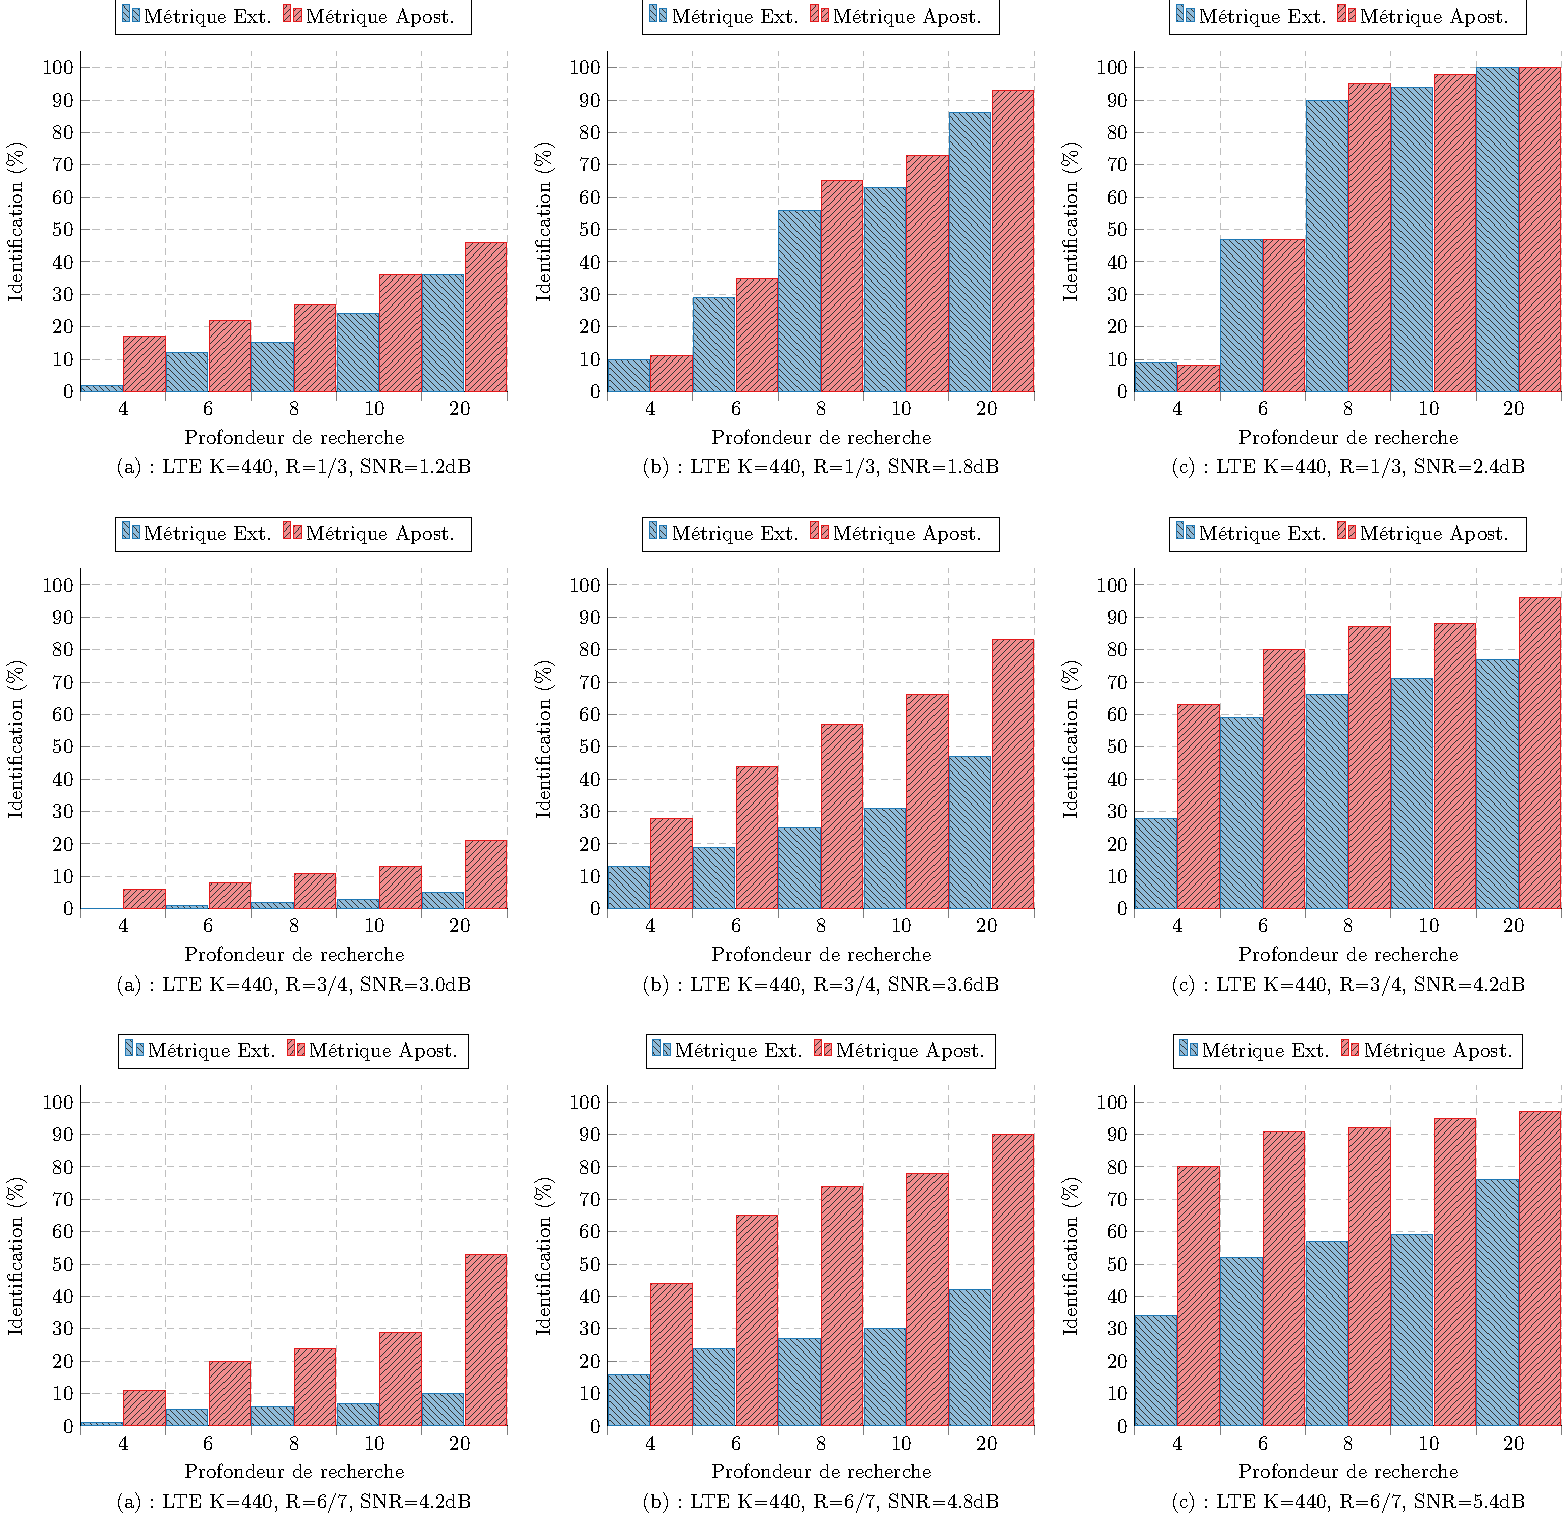
\includegraphics[width=1.05\textwidth]{main/ch3_fig/id2/dvb/tikz/440.pdf}
	\caption{Pourcentage d'identification pour différents turbo codes du standard DVB-RCS K=440, R=1/3, 3/4 et 6/7.
	Décodage EML-MAP itérant 8 fois. \label{fig:dvb440}}
\end{figure}